\documentclass[12pt,a4paper]{article}
\usepackage[utf8]{inputenc}
\usepackage[T1]{fontenc}
\usepackage[english,brazilian]{babel}
\usepackage{amsmath}
\usepackage{amsthm}
\usepackage{amsfonts}
\usepackage{amssymb}
\usepackage{graphicx}
\usepackage{indentfirst}
\usepackage[normalem]{ulem}
\usepackage{setspace}
\usepackage{hyperref}
\usepackage{lipsum}
\usepackage{multicol}
\usepackage{quoting}
\usepackage{blindtext}
\usepackage{caption}
\usepackage{xcolor}
\usepackage{xwatermark}
\newwatermark[allpages,angle = 60, scale = 2.5, color = red!5]{Mauro José Silva Sousa}
\usepackage[left=3.00cm, right=2.00cm, top=3.00cm, bottom=2.00cm]{geometry}

\begin{document}
    \onehalfspacing
    \thispagestyle{empty}
    
    \begin{center}
        \includegraphics[scale = .90]{Relatorio de fisica experimental/UFCG.png}

        \vspace{4cm}

        \textbf{Mauro José Silva Sousa}
    \end{center}
        
    
    \vspace{4cm}
    
    \begin{center}
        \textbf{\Huge Missão 4.0: Hand Tracking}
    \end{center}

    \vspace{8cm}
    \begin{center}
        Campina Grande

        \today
    \end{center}
    \newpage
    \tableofcontents
    \thispagestyle{empty}
    \newpage

    \pagestyle{headings}
    \section*{INTRODUÇÃO}
    \addcontentsline{toc}{section}{INTRODUÇÃO}

        O reconhecimento de gestos da mão é uma tarefa desafiadora em visão computacional. Neste projeto, foi desenvolvido um sistema de reconhecimento de números utilizando os dedos da mão. Utilizamos ferramentas como OpenCV e mediapipe para detectar a mão e identificar os dedos, e em seguida, realizamos o reconhecimento de padrões para determinar o número que estava sendo exibido pelos dedos. Este relatório apresentará a metodologia utilizada, os resultados alcançados e as limitações encontradas durante o desenvolvimento do projeto.

        O OpenCV (Open Source Computer Vision Library) é uma biblioteca de código aberto que fornece ferramentas para processamento de imagens e visão computacional. É uma das bibliotecas mais utilizadas na área de visão computacional devido à sua facilidade de uso e suporte a várias linguagens de programação, como Python e C++. 

        O mediapipe é uma biblioteca de visão computacional desenvolvida pelo Google que fornece ferramentas para processamento de imagem e detecção de pontos-chave (landmarks) em imagens e vídeos. A biblioteca oferece modelos pré-treinados para detectar poses humanas, gestos da mão e outras tarefas de reconhecimento de padrões.
    
    \newpage

    \section{OBJETIVOS DO PROJETO}

        Esse projeto tem como objetivo o desenvolvimento de uma aplicação utilizando as bibliotecas OpenCV e MediaPipe para realizar o reconhecimento de números utilizando os dedos da mão. A aplicação irá detectar a mão e identificar a posição dos dedos usando a biblioteca MediaPipe. Em seguida, um algoritmo será implementado para reconhecer a quantidade de dedos levantados e identificar o número correspondente.

        O objetivo é obter um bom desempenho na detecção dos dedos e na identificação dos números, com um limite de erro aceitável e um tempo de resposta rápido. Além disso, o projeto tem o objetivo de demonstrar as habilidades de visão computacional e programação em python com o OpenCV e MediaPipe.

    \newpage

    \section{METODOLOGIA}

        Para a criação de uma aplicação com o OpenCV, utilizando a classe VideoCapture do OpenCV. Essa classe permite acessar o fluxo do video da camera e ler cada frame da imagem. Foi preciso criar um objeto da classe VideoCapture.

        Aplicamos técnicas de pré-processamento de imagem, como a redução de ruídos e a equalização, para melhorar a qualidade do fluxo de vídeo com o OpenCV, utilizando tecnicas de pre-processamento de imagem, redução de ruidos e equalização.

        Utilizando a biblioteca MediaPipe para detectar a palma da mão e identificar a posição dos dedos na imagem usando um modelo pre-treinado.

        Desenvolvemos algoritmos para reconhecer a quantidade de dedos levantados e identificar o número correspondente.

        Utilizamos a classe HandoLandmark do MediaPipe para inferir os pontos-chaves da mão, como mostra a imagem abaixo:

        \begin{figure}[!h]
            \centering
            \caption{HandLandmark}
            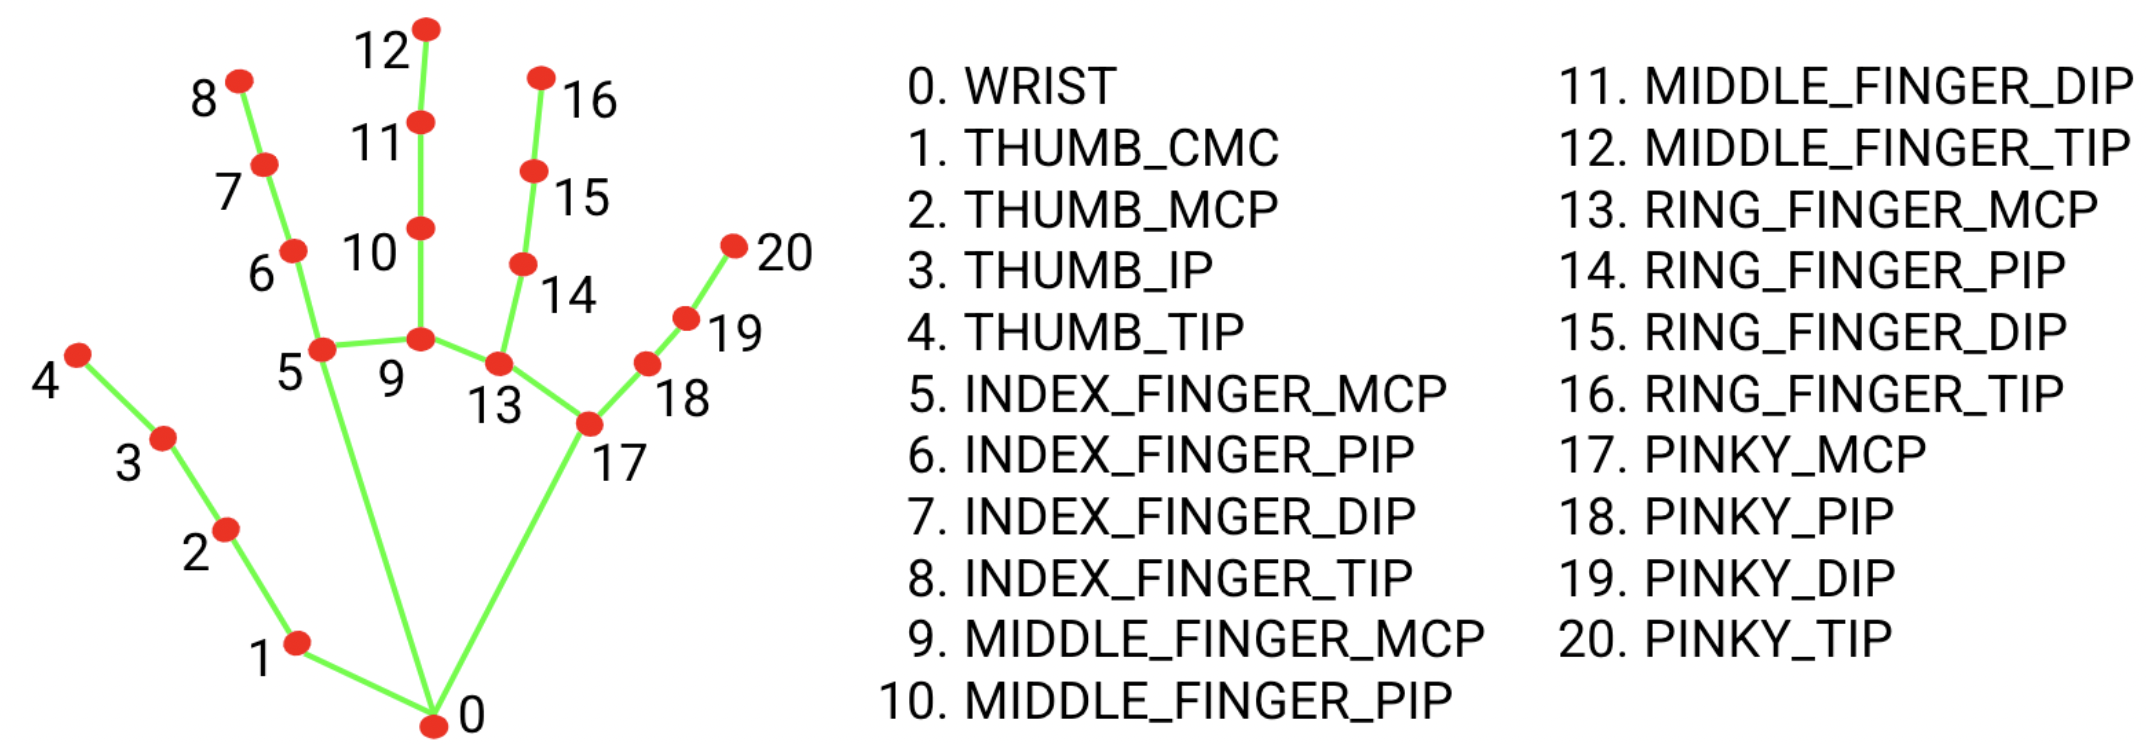
\includegraphics[scale=.3]{RAS Teste/Ras Missão 4.0/mao.png}
            \caption*{Fonte: Imagem tirada do site \href{https://developers.google.com/mediapipe/solutions/vision/hand_landmarker}{MediaPipe}}
            \label{fig:my_label}
        \end{figure}

        Como a rede neural, ja vem pre-treinado com o MediaPipe. Foi facil inferir os landmarks da mão no video.

        Usando a classe hands do MediaPipe para aplicar a detecção da palma da mão em tempo real. Essa classe usa o modelo do HandLandmark.


    \newpage

    \section{RESULTADOS OBTIDOS}
    
        Durante o processo de desenvolvimento da aplicação de reconhecimento de números utilizando os dedos da mão, encontramos algumas dificuldades que exigiram soluções criativas e bem cuidadosas para garantir o sucesso do projeto.

        Um dos primeiros desafios foi a calibração adequada da detecção dos dedos. Para resolver esse problema, realizamos testes e ajustes frequentes no código, tornando-o mais adaptável e sensível às características individuais.

        Outro obstáculo foi a precisão da detecção dos dedos, que em alguns casos apresentou falhas e inconsistências, afetando o reconhecimento correto dos números. Para contornar essa questão, fizemos ajustes no código, além de testes e validações com diferentes usuários, garantindo assim a eficácia do sistema em diferentes condições e cenários.

        Durante o processo de integração da biblioteca MediaPipe para detecção da palma da mão, encontramos dificuldades na configuração e utilização da ferramenta. Foi necessário um estudo mais aprofundado e a busca por informações adicionais na documentação da biblioteca.

        Apesar desses desafios, o resultado final da aplicação foi satisfatório, apresentando um bom desempenho na detecção dos dedos e reconhecimento dos números em diferentes cenários e condições de iluminação.

        \newpage
        
    
    \section*{CONCLUSÃO}
    \thispagestyle{myheadings}
    \markright{ }
    \addcontentsline{toc}{section}{CONCLUSÃO}

        As técnicas de processamento de imagem e reconhecimento de padrões exploradas neste projeto têm o potencial de serem aplicadas em diversas áreas além do reconhecimento de números utilizando os dedos da mão. Por exemplo, essas técnicas podem ser usadas para controlar dispositivos eletrônicos, como robôs e drones, e para desenvolver interfaces de usuário mais intuitivas e naturais.

        Além da detecção precisa de números, este projeto demonstrou a importância de considerar diferentes condições de iluminação e fundos complexos em futuras implementações. Ao longo do desenvolvimento, descobrimos que essas condições podem impactar negativamente a precisão da detecção, o que deve ser levado em consideração ao explorar aplicações mais complexas.

        Considerando os objetivos propostos e as limitações encontradas, este projeto foi bem-sucedido em seu propósito e trouxe aprendizados importantes para o desenvolvimento de aplicações de visão computacional. Além disso, é claro que a tecnologia desenvolvida neste projeto tem o potencial de ser aplicada em diversas áreas, como na automação de processos industriais e na área da saúde, como ferramenta para o auxílio no diagnóstico de doenças que afetam a coordenação motora das mãos.

    \section*{REFERENCIA}
    \addcontentsline{toc}{section}{REFERÊNCIA}

        \noindent OpenCV Documentation. Disponível em: \url{https://docs.opencv.org/master/}. Acessado em: 25 de março de 2024.
        
        \noindent Mediapipe Documentation. Disponível em: \url{https://developers.google.com/mediapipe/solutions/vision/hand_landmarker}. Acessado em: 25 de março de 2024.

        \noindent ANTONELLO, Ricardo. \textbf{Introdução a Visão Computacional com Python e OpenCV.} Versão 0.8 - Não corrigida. Florianopolis: Ricardo Antonello, 2015.

        
\end{document}